% Panel (c): oxygen transport across the oxide and the interfacial reactions.
% Canvas ~9 x 6 cm, 10 pt, styled to match panels (a) and (b).
% Text positions are set from measured label widths (\settowidth), not by eye.
\documentclass[12pt,border=2pt,tikz]{standalone}

\usepackage{amsmath}

\newcommand{\lat}{\mathrm{lat}}
\newcommand{\ox}{\mathrm{ox}}
\newcommand{\Ox}{\mathrm{O}}

\usetikzlibrary{arrows.meta}

\definecolor{cOx}{RGB}{250,224,80}
\definecolor{cMetal}{RGB}{214,214,211}
\definecolor{cEdge}{RGB}{40,40,44}
\definecolor{cAcc}{RGB}{20,72,124}
\definecolor{cGB}{RGB}{96,42,140}
\definecolor{cRed}{RGB}{158,54,42}

\begin{document}
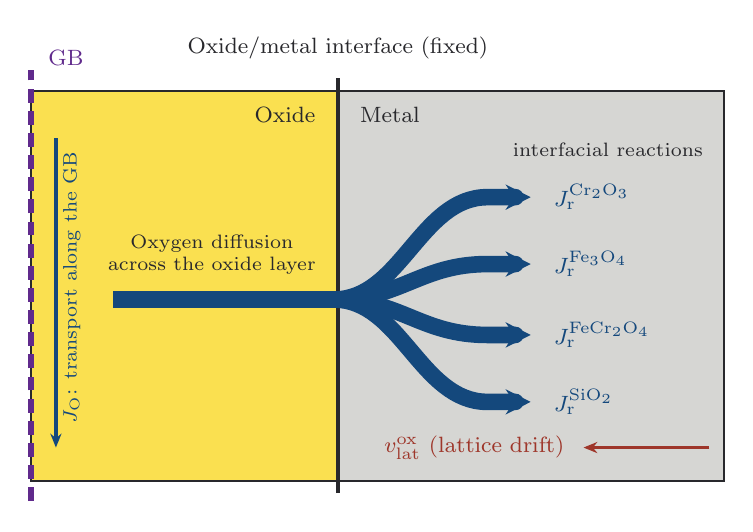
\begin{tikzpicture}[
  x=1cm,y=1cm, font=\footnotesize, color=cEdge,
  eg/.style    ={draw=cEdge, line width=0.8pt},
  odiff/.style ={-{Stealth[length=5pt,width=4pt]}, line width=1.25pt, draw=cAcc},
  drift/.style ={-{Stealth[length=5pt,width=4pt]}, line width=1.1pt, draw=cRed},
  key/.style   ={font=\scriptsize, color=cEdge},
]

\def\W{8.80}\def\H{4.95}\def\xI{3.90}

% ----- oxide and metal --------------------------------------------------
\fill[cOx]    (0,0)   rectangle (\xI,\H);
\fill[cMetal] (\xI,0) rectangle (\W,\H);
\draw[eg]     (0,0)   rectangle (\W,\H);

% ----- the two boundaries -----------------------------------------------
\draw[cGB,line width=2.2pt,dash pattern=on 5pt off 3pt] (0,-0.26) -- (0,\H+0.26);
\draw[cEdge,line width=1.6pt] (\xI,-0.16) -- (\xI,\H+0.16);
\node[anchor=west,cGB] at (0.10,\H+0.42) {GB};
\node[anchor=south]    at (\xI,\H+0.28)  {Oxide/metal interface (fixed)};

% ----- region labels: mirrored about the interface ----------------------
\node[anchor=east] at (\xI-0.16,\H-0.30) {Oxide};
\node[anchor=west] at (\xI+0.16,\H-0.30) {Metal};

% ----- oxygen arriving along the GB -------------------------------------
\draw[odiff] (0.32,4.35) -- (0.32,0.42);
\node[cAcc,font=\scriptsize,rotate=90] at (0.52,2.45)
      {$J_{\Ox}$: transport along the GB};

% ----- one split arrow: smooth fan, ends parallel -----------------------
\draw[cAcc,line width=6pt,line cap=butt] (1.05,2.30) -- (4.05,2.30);
\foreach \yy in {3.60,2.75,1.85,1.00}{
  \draw[cAcc,line width=6pt,line cap=round,
        -{Stealth[length=9pt,width=9pt]}]
    (3.85,2.30) .. controls (4.70,2.30) and (4.95,\yy) .. (5.80,\yy)
    -- (6.35,\yy);}

% centred at 2.30: the free span runs from the rotated label (0.70) to \xI
\node[key,anchor=south,align=center] at (2.30,2.50)
      {Oxygen diffusion\\ across the oxide layer};

\node[key,anchor=east]  at (8.66,4.20) {interfacial reactions};
\node[anchor=west,cAcc] at (6.52,3.60) {$J_{\mathrm{r}}^{\mathrm{Cr_2O_3}}$};
\node[anchor=west,cAcc] at (6.52,2.75) {$J_{\mathrm{r}}^{\mathrm{Fe_3O_4}}$};
\node[anchor=west,cAcc] at (6.52,1.85) {$J_{\mathrm{r}}^{\mathrm{FeCr_2O_4}}$};
\node[anchor=west,cAcc] at (6.52,1.00) {$J_{\mathrm{r}}^{\mathrm{SiO_2}}$};

% ----- metal consumed: the lattice drifts towards the interface ---------
% label is 2.66 cm wide; anchored at 6.90 it clears the interface by 0.34 cm
\draw[drift] (8.62,0.42) -- (7.02,0.42);
\node[anchor=east,cRed] at (6.90,0.42) {$v_{\lat}^{\ox}$ (lattice drift)};

\end{tikzpicture}
\end{document}
